%%%%%%%%%%%%%%%%%%%%%%%%%%%%%%%%%%%%%%%%%%%%%%%%%%%%
\documentclass[a4paper,fleqn,10pt,twocolumn]{SICE_ISCS}
%\usepackage{url}
\usepackage{ascmac}
\usepackage{amssymb}
%\usepackage{amsmath}
%\usepackage{hyperref}
%\usepackage{lmodern}
\usepackage{breqn}
\usepackage{bm}
\usepackage{comment}
\usepackage{pdfpages}
%\usepackage{HERE}
%\usepackage[version=3]{mhchem}%%化学式
%\usepackage{siunitx}
\usepackage[utf8]{inputenc}
\newcommand{\Tabref}[1]{{Table~\ref{#1}}}
\newcommand{\Equref}[1]{式(\ref{#1})}
\newcommand{\Figref}[1]{{Fig.~\ref{#1}}}
\newcommand{\blue}[1]{\textcolor{blue}{#1}} 
\title{Collaborative Localization of UAVs in Monotone Environments\\
	 Using Stein Particle Filters}

\author{Tomoki Arita${}^{1\dagger}$ and Toru Namerikawa${}^{2}$}
% The dagger symbol indicates the presenter.
\speaker{Tomoki Arita}

\affils{${}^{1}$School of Integrated Design Engineering, Keio University, Kanagawa, Japan\\
	    ${}^{2}$Department of System Design Engineering, Keio University, Kanagawa, Japan\\
(Tel: +81-45-563-1151; E-mail: arita@keio.jp, namerikawa@sd.keio.ac.jp)\\
}
\abstract{%
In extensive and monotonous outdoor environments such as farmlands and forest areas, global self-localization through image matching often fails due to error accumulation and outlier effects. Particularly in cooperative estimation involving multiple agents, there is a need to efficiently solve multi-modal combination problems to construct a unified relative position graph. In this study, we propose a Cooperative Visual Inertial System (CoVINS) method that incorporates position-based likelihood into conventional image feature matching using the Stein Particle Filter. By combining Stein Variational Gradient Descent with Relaxed ADMM, our approach enables robust collaborative localization even in environments with high outlier rates. Simulation results demonstrate that the proposed method can maintain accurate localization with outlier rates up to 50\%, and real-world experiments confirm its effectiveness in practical scenarios.}

\keywords{%
Collaborative localization, Stein particle filter, Visual inertial system, Multi-agent systems, Outlier robustness.
}

\begin{document}

\maketitle

%-----------------------------------------------------------------------

\section{Introduction}
Many autonomous mobile robots require self-localization as the foundation for their operation. With the increasing integration of autonomous robots into society, self-localization technologies for harsh environments and mountainous regions where GPS/GNSS is unavailable have been extensively researched. Self-localization consists of two hierarchical levels: local self-localization used for dynamic control and local motion planning, and global self-localization used for creating consistent environmental maps and wide-area path planning. In environments where GPS/GNSS is unavailable, global self-localization is typically achieved by structuring point cloud and image data obtained from LiDAR, cameras, and other sensors through various matching methods. In practical applications, Visual Inertial Systems (VINS), which combine cameras and Inertial Measurement Units (IMUs), are widely used due to their cost-effective hardware implementation\cite{VINS-Mono}.

Furthermore, with the proliferation of autonomous mobile robots, multi-agent environments where multiple agents operate simultaneously have become a major research area in recent years. Even in harsh environments and mountainous regions where GPS/GNSS is unavailable, collaborative work by multiple agents has been attempted in several studies from the perspectives of system-wide fault tolerance and scalability for respective objectives\cite{Multi-Robot-SLAM,Swarm-Robots}.

Given these backgrounds, while global self-localization methods without GPS/GNSS are in demand, in monotonous and vast outdoor environments such as farmlands and forests, global self-localization through image matching often fails due to error accumulation and outlier effects. Especially in cooperative estimation involving multiple agents, as each agent's erroneous state estimation affects all agents, the probability of the entire system making incorrect estimations increases exponentially with the proportion of outliers for each agent. Therefore, in this research, we propose a VINS method that considers likelihood based on position information in addition to conventional image feature matching using Stein Particle Filter, and achieves consensus on estimated states among multiple agents.

\section{Collaborative Visual Inertial System}
The Collaborative Visual Inertial System (CoVINS) for cooperative self-localization is structured as shown in Fig. \ref{fig:covins}. There are $N$ agents equipped with cameras and IMUs, and each agent transmits the image information observed by its camera to adjacent agents. The agent receiving the image information searches within its database, detects images that have observed the same landmark, and sends back the relative position between the camera frames in the two images. In the context of graph optimization, each agent creates a pose graph, which is a graph of relative positions, using the obtained relative position information\cite{Factor-Graphs}. If a pose graph that reproduces each obtained relative position can be generated as a result of optimization, it can be said that a consistent position estimation has been achieved.

\begin{figure}[t]
	\begin{center}
		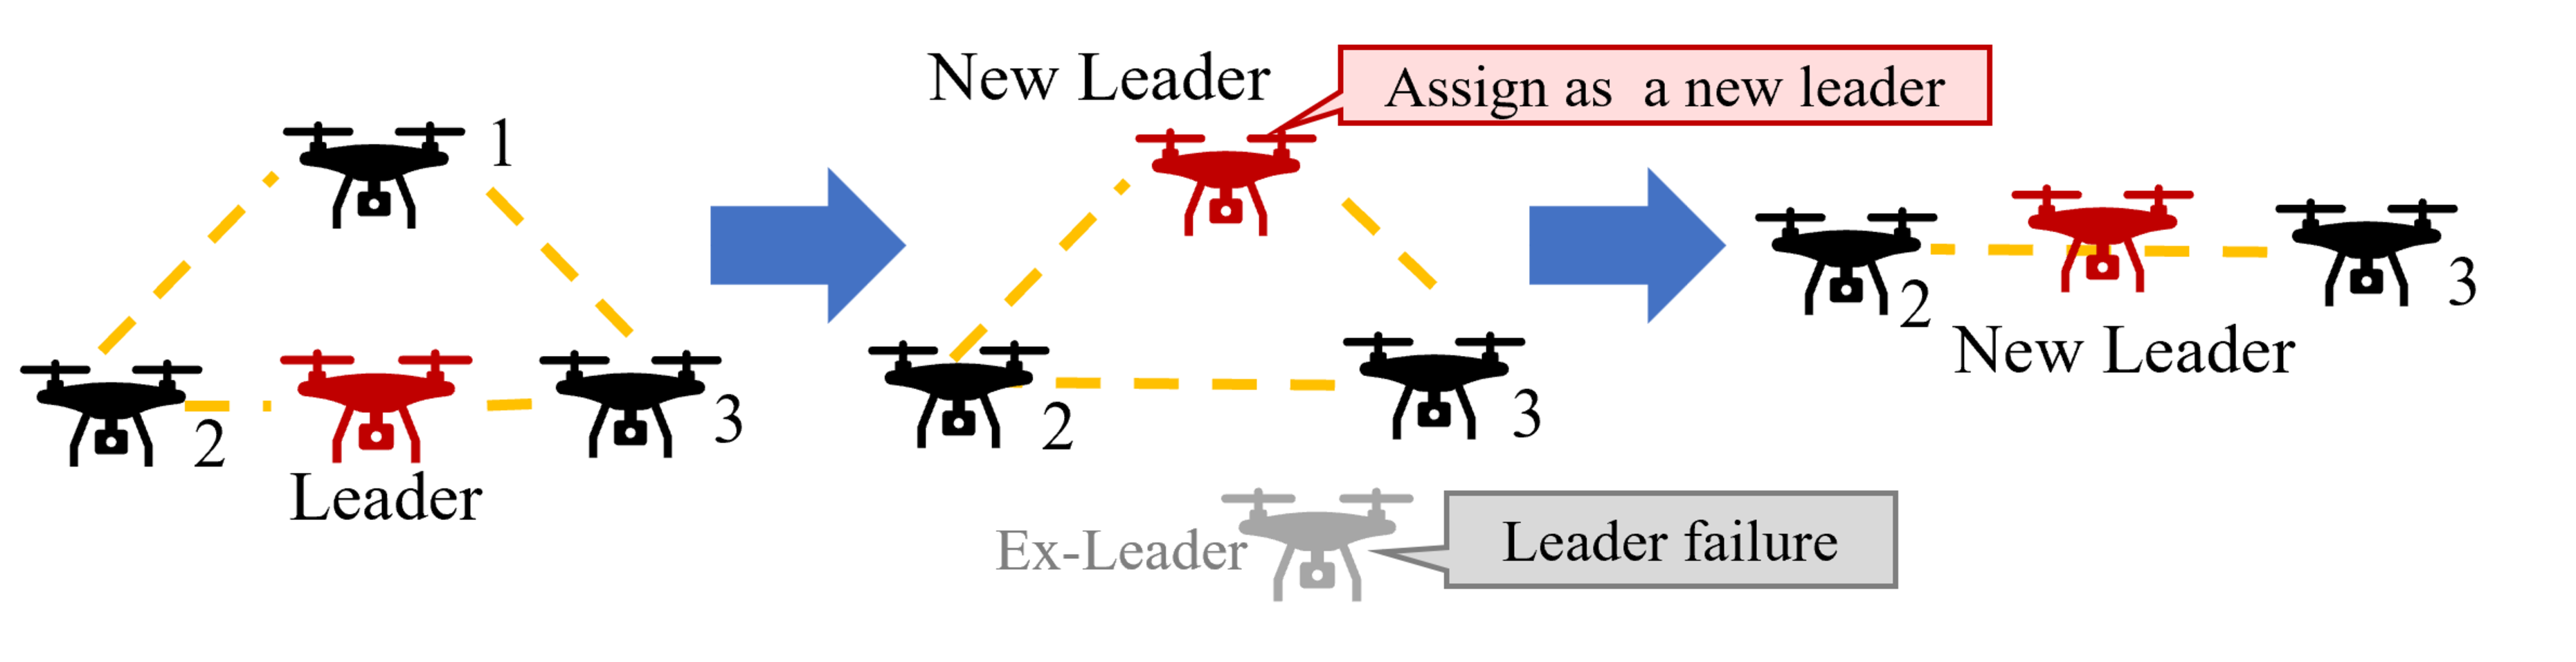
\includegraphics[width=\linewidth]{Fig/Nice_image_fault.eps}
		\caption{Collaborative Visual Inertial System (CoVINS).}
		\label{fig:covins}
	\end{center}
	\vspace{-2mm}
\end{figure}

On the other hand, in uneven environments such as farms and forests, global self-localization through optimization does not function sufficiently. The cause of this is believed to be that similar image matching does not function in monotonous environments, resulting in incorrect matching on the pose graph. From these backgrounds, a simplified model as shown in Fig. \ref{fig:primitive_model} can be considered. In Fig. \ref{fig:primitive_model}, the red and black circles represent nodes indicating the positions of each agent, and the black lines represent edges. In the ideal environment of Fig. \ref{fig:primitive_model}(a), the graph can be optimized by generating edges, but in the case of Fig. \ref{fig:primitive_model}(b) where correct and incorrect edges exist, the optimization results in selecting the internal division point of the two, which is an undesirable result considering the problem setting. Here, a motivation arises that by using a particle filter, it might be possible to simultaneously explore two graphs that could be generated by correct and incorrect edges, as shown in Fig. \ref{fig:primitive_model}(c). From this point, this paper attempts to reformulate factor graphs from the perspective of particle filters.

\begin{figure}[t]
	\begin{center}
		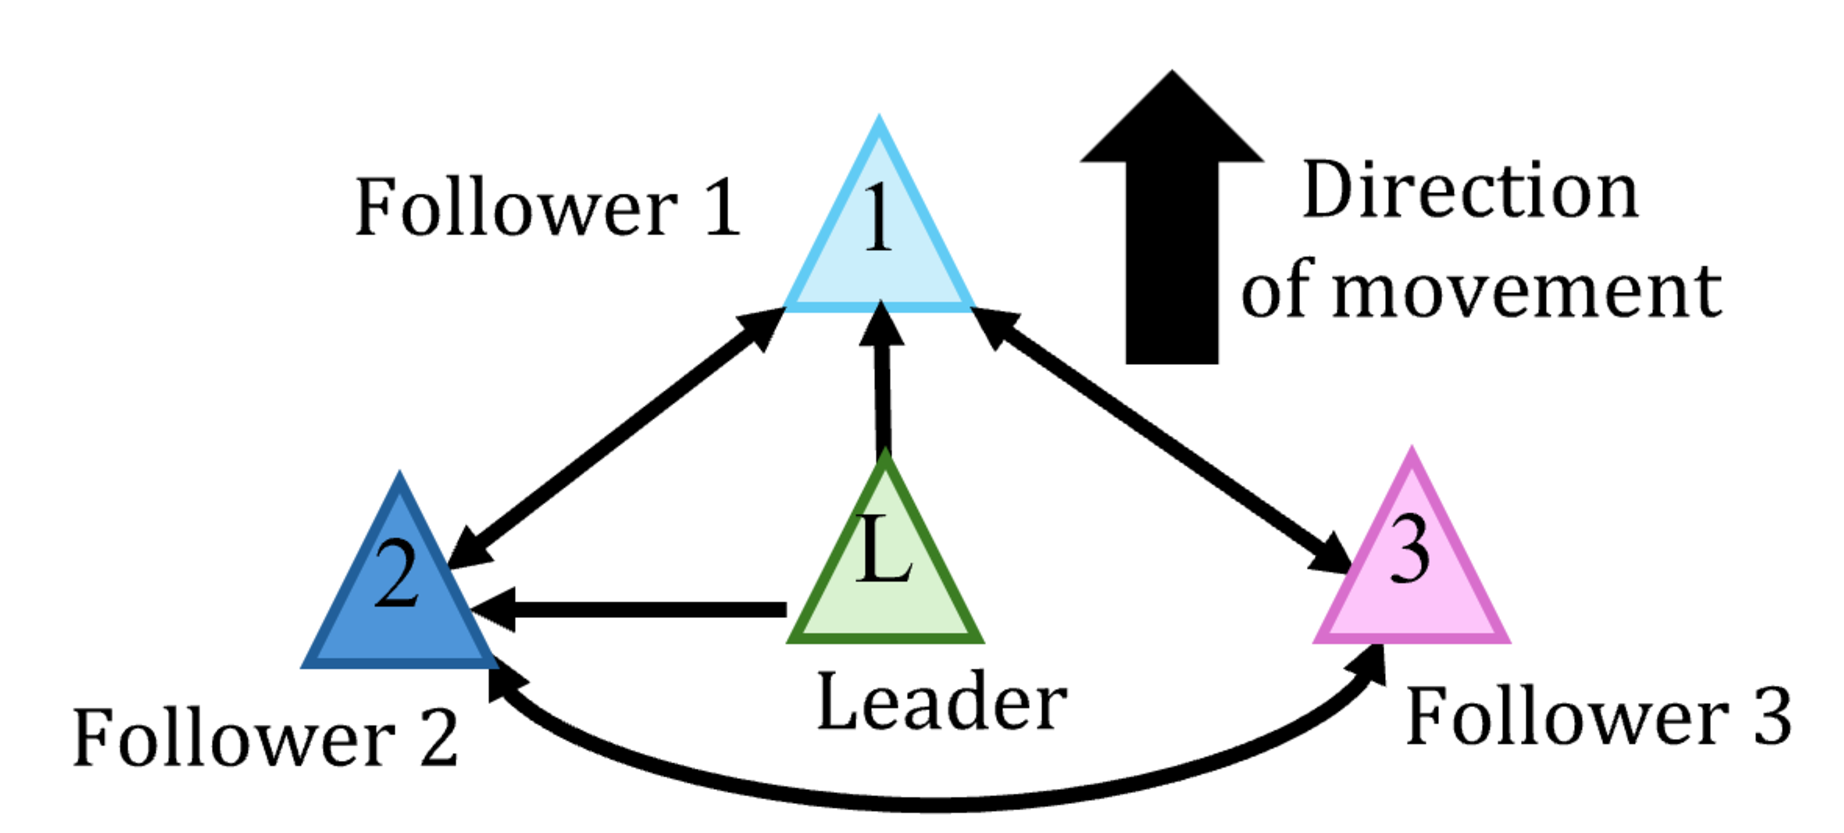
\includegraphics[width=\linewidth]{Fig/Topology.eps}
		\caption{Primitive model of factor graph: (a) case 1 - ideal environment with correct edges, (b) case 2 - environment with both correct and incorrect edges, (c) case 3 - simultaneous exploration of multiple possible graphs.}
		\label{fig:primitive_model}
	\end{center}
	\vspace{-2mm}
\end{figure}

\section{Mathematical Preliminaries}
\subsection{Representation of Three-Dimensional Rotation}
In this paper, we perform 6 degrees of freedom state estimation, which involves operations on three-dimensional rotations. The three-dimensional special orthogonal group $\mathrm{SO}(3)$ representing three-dimensional rotations, the three-dimensional special Euclidean group $\mathrm{SE}(3)$ adding translation, and their product $\otimes$ cannot be calculated on vector spaces, so adaptations are necessary to enable differentiation and other operations. Here, following the literature\cite{VINS-IMU}, we define mappings to and from vector spaces, inverse mappings, and operators for arbitrary operations in $\mathrm{SO}(3)$ and $\mathrm{SE}(3)$. $\mathrm{SO}(3)$ forms a Lie group and can be converted to the corresponding Lie algebra $\mathrm{so}(3)$ and vectors in linear space by the following exponential and logarithmic mappings.

\begin{equation}
\begin{aligned}
& \log : \mathrm{SO}(3) \rightarrow \mathbb{R}^{3} \\
& \exp : \mathbb{R}^{3} \rightarrow \mathrm{SO}(3) \\
& \left(\cdot\right)^{\circ}: \mathrm{so}(3) \rightarrow \mathbb{R}^{3} \\
& \left(\cdot\right)^{\wedge}: \mathbb{R}^{3} \rightarrow \mathrm{so}(3)
\end{aligned}
\end{equation}

Similarly for $\mathrm{SE}(3)$:

\begin{equation}
\begin{aligned}
& \log : \mathrm{SE}(3) \rightarrow \mathbb{R}^{6} \\
& \exp : \mathbb{R}^{6} \rightarrow \mathrm{SE}(3)
\end{aligned}
\end{equation}

Also, $T \in \mathrm{SE}(3)$ can be matrix-decomposed using the translation $\mathbf{t} \in \mathbb{R}^{3}$ and the rotation $\mathbf{R} \in \mathrm{SO}(3)$ as follows:

\begin{equation}
T=\left(\begin{array}{c|c}
\mathbf{R} & \mathbf{t} \\
\hline \mathbf{0} & 1
\end{array}\right)
\end{equation}

We define $\oplus: \mathrm{SE}(3) \times \mathbb{R}^{3} \rightarrow \mathbb{R}^{3}$ as:

\begin{equation}
\theta, p \mapsto \mathbf{R}(\theta) p+\mathbf{t}(\theta)
\end{equation}

\subsection{Relaxed ADMM}
The cooperative self-localization addressed in this paper can be formulated as a convex optimization problem with consensus constraints. In this case, the original problem can be solved as an approximation problem in the dual space using Relaxed ADMM (Alternating Direction Method of Multipliers)\cite{ADMM}.

The constrained optimization problem:

\begin{equation}
\begin{aligned}
& \min _{x, y} f(x)+g(y) \\
& \text { s.t. } A x+B y=b
\end{aligned}
\end{equation}

can be solved by transforming it into a relaxation problem that minimizes the following Lagrangian:

\begin{equation}
\mathcal{L}(x, y, z)=f(x)+g(y)+z^{T}(b-A x-B y)
\end{equation}

where $z$ is the dual variable. On the other hand, when the Lagrangian cannot be directly minimized, the original problem can be solved by maximizing the Lagrangian dual function:

\begin{equation}
\begin{aligned}
d(z) & =\inf _{x, y}\left\{f(x)+g(y)+z^{T}(b-A x-B y)\right\} \\
& =\inf \{f(x)-\langle z, A x\rangle\}+\inf _{y}\{g(y)-\langle z, B y-b\rangle\} \\
& =\inf \mathcal{L}_{f}(z)+\inf _{y} \mathcal{L}_{g}(z)
\end{aligned}
\end{equation}

In Relaxed ADMM, from the context of equation (7), the solution to equation (5) can be obtained by calculating as follows:

\begin{equation}
\begin{aligned}
& y^{+}=\underset{y}{\arg \min } \mathcal{L}_{g, y}(z) \\
& \omega_{g}=z-\gamma\left(B y^{+}-b\right) \\
& x^{+}=\underset{x}{\arg \min } \mathcal{L}_{f, y}\left(2 \omega_{g}-z\right) \\
& \omega_{f}=2 \omega_{g}-z-\gamma A x^{+} \\
& z^{+}=z+\eta\left(\omega_{f}-\omega_{g}\right)
\end{aligned}
\end{equation}

where $\mathcal{L}_{f, y}$ and $\mathcal{L}_{g, y}$ are the extended Lagrangians:

\begin{equation}
\begin{aligned}
& \mathcal{L}_{f, y}(z)=f(x)-\langle z, A x\rangle+\frac{\gamma}{2}\|A x\|^{2} \\
& \mathcal{L}_{g, y}(z)=g(y)-\langle z, B y-b\rangle+\frac{\gamma}{2}\|B y-b\|^{2}
\end{aligned}
\end{equation}

\subsection{Stein Variational Gradient Descent}
Consider the following minimization problem of the Kullback-Leibler divergence:

\begin{equation}
q^{*}=\underset{q \in Q}{\arg \min }\left\{D_{K L}(q \| p) \equiv \mathbb{E}_{q}[\log q(x)]-\mathbb{E}_{q}[\log p(x)]\right\}
\end{equation}

The following theorem holds:

\textbf{Theorem 1} (Relationship between KL divergence and Stein Operator\cite{SVGD}). For a transformation $\boldsymbol{T}(x)=x+\epsilon \phi(x)$, when $x \sim q(x)$, if the probability distribution of $z=\boldsymbol{T}(x)$ is denoted as $q_{(\boldsymbol{T})}(z)$, then:

\begin{equation}
\nabla_{\epsilon} D_{K L}\left(\left.q_{(\boldsymbol{T})} \| p\right)\right|_{\epsilon=0}=-\mathbb{E}_{x \sim q}\left\{\mathcal{A}_{p} \phi(x)\right\}
\end{equation}

holds, where $\mathcal{A}_{p} \phi(x)=\nabla_{x} \log p(x) \phi(x)^{\mathrm{T}}+\nabla_{x} \phi(x)$ is the Stein Operator, and $\phi$ is a functional belonging to the reproducing kernel Hilbert space $\mathcal{H}^{d}$.

Here, if we define the Kernelized Stein Discrepancy (KSD) as:

\begin{equation}
\mathbb{D}(q, p)=\max _{\phi \in \mathcal{H}^{d}} \mathbb{E}_{x \sim q}\left[\mathcal{A}_{p} \phi(x)\right], \quad \text { s.t. } \quad\|\phi\|_{\mathcal{H}} \leq 1
\end{equation}

the solution to this problem is given by:

\begin{equation}
\phi_{q, p}^{*}(\cdot)=\mathbb{E}_{x \sim q}\left[k(x, \cdot) \nabla_{x} \log p(x)+\nabla_{x} k(x, \cdot)\right]
\end{equation}

\section{Problem Formulation}
Cooperative self-localization can be formulated as the following maximum a posteriori probability estimation problem (MAP estimation problem), where the state of agent $i$ at time step $t$ is $x_{i}^{t}$, and the observations of each agent are $z_{t}=\left\{z_{t}^{1}, \cdots, z_{t}^{N}\right\}$:

\begin{equation}
\max _{x_{1}^{t+1}, \cdots, x_{N}^{t+1}} \sum_{i=1}^{N} P\left(x_{i}^{t+1} \mid Z_{t}\right) Q\left(z_{t+1} \mid x_{i}^{t+1}\right)
\end{equation}

Here, the distribution $P$ represents the probability distribution of agent $i$'s state before the observation information $z_{t}$ is given at time step $t$, and the distribution $Q$ represents the likelihood distribution of obtaining the observation information $z_{t}$ at state $x_{i}$. Also, $Z_{t}=\left[z_{0}, \cdots, z_{t}\right]$.

\section{Stein Particle Filter}
The Stein Particle Filter (SPF) is a method for numerically analyzing non-Gaussian and nonlinear probabilistic state estimation problems, with its basic framework proposed in the literature\cite{SPF}. In SPF, probability distributions are represented by particle sets, which are updated using a gradient method based on Stein Variational Gradient Descent (SVGD).

While traditional particle filters may suffer from particle degradation due to resampling, SPF smoothly transforms the particle distribution using SVGD and converges it to the target distribution. SVGD executes the minimization of the Kullback-Leibler information amount (KL divergence) using an operator called the Stein operator. Here, considering:

\begin{equation}
q^{*}=\underset{q}{\arg \min } D_{K L}(q \| p)
\end{equation}

by formulating variational inference to converge from $q$ to $p$ using the Stein operator as in equation (11), particles can be moved according to the gradient to approach $p$.

Equation (14) is difficult to solve analytically using methods like the Kalman filter when $P$ cannot be assumed to be a Gaussian distribution. In the Stein Particle Filter, the distribution $P\left(x_{i} \mid Z_{t}\right)$ is approximated as:

\begin{equation}
P\left(x_{i} \mid Z_{t}\right)=\frac{1}{m} \sum_{j=1}^{m} P\left(x_{j}^{t} \mid Z_{t}\right)
\end{equation}

using a set of particles $\mathcal{X}=\left\{x_{i}^{t}\right\}_{i=1}^{m}$, and by moving each particle according to the gradient method, the MAP estimation problem can be solved without algebraic approximation of the probability distribution. Like various filtering methods, the Stein Particle Filter is divided into a prediction step that calculates $P\left(x_{t+1} \mid z_{t}\right)$ and an update step that calculates $Q\left(z_{t+1} \mid x_{t+1}\right)$, as described below.

\subsection{Calculation of $P\left(x_{t+1} \mid z_{t}\right)$ (Prediction Step)}
In the prediction step, it is necessary to calculate $P\left(x_{t+1} \mid z_{t}\right)$ in equation (14). This is an operation to predict the state at step $t+1$ from the information up to step $t$, and in VINS, it is obtained by numerically integrating the acceleration $a_{m}$ and angular velocity $\omega_{m}$ obtained from the IMU. Numerical integration on $\mathrm{SE}(3)$ can be calculated using a framework similar to the literature\cite{On-Manifold} as follows:

\begin{equation}
\begin{aligned}
p_{k+1}= & p_{k}+v_{k} \Delta t \\
& +\int \int_{i \in\left\{z_{t}, i_{t+1}\right\}} \frac{\left\{R_{k}\left(a_{m}-b_{n}-\eta_{m d}\right)+g\right\} d t^{2}}{\dot{a}} \\
v_{k+1}= & v_{k}+\int_{i \in\left\{z_{t}, i_{t+1}\right\}} \dot{a} d t \\
R_{k+1}= & R_{k} \otimes \exp \left(\int_{i \in\left\{z_{t}, i_{t+1}\right\}} \frac{\left(\omega_{m}-b_{g}-\eta_{g d}\right) d t}{\dot{\omega}}\right)
\end{aligned}
\end{equation}

where $p$ is position, $v$ is velocity, $R$ is the rotation matrix representing attitude, $b_{n}$ and $b_{g}$ are the biases of acceleration and angular velocity respectively, and $\eta_{m d}$ and $\eta_{g d}$ are white noise. Each particle is updated by the transformation ${ }^{t} T_{t+1} \in \mathrm{SE}(3)$ obtained by numerical integration as follows:

\begin{equation}
\bar{x}_{t+1}^{i}=x_{i}^{t} \otimes^{t} T_{t+1}, \forall i
\end{equation}

\subsection{Calculation of $Q\left(z_{t+1} \mid x_{t+1}\right)$ (Update Step)}
In the update step, it is necessary to calculate the likelihood $Q\left(z_{t+1} \mid x_{t+1}\right)$, which represents the plausibility of the observation, and to transform the prediction distribution $P\left(x_{t+1} \mid z_{t}\right)$ by some method. In the Stein Particle Filter, equation (14) is replaced with the KL divergence minimization problem:

\begin{equation}
\begin{aligned}
& \max _{x_{t+1}^{i}} P\left(x_{t+1}^{i} \mid Z_{t}\right) Q\left(z_{t+1} \mid x_{t+1}\right) \\
& =\max _{x_{t+1}^{i}} \underset{P_{Q T}}{\arg \min } D_{K L}\left(P\left(x_{t+1}^{i} \mid Z_{t}\right)_{\left[T_{i}\right]} \| P_{Q}\right)
\end{aligned}
\end{equation}

Furthermore, by changing the formulation of equation (18) to variational inference, the MAP solution can be obtained as follows:

\begin{equation}
\begin{aligned}
\min _{P_{i}(x)} \nabla_{x} D_{K L}\left(P\left(x_{i+1}^{j} \mid Z_{i}\right)_{\left[T_{i}\right]} \| P_{Q_{i}}\right)_{\mid \epsilon=0} \\
\Rightarrow T:=T \oplus \phi^{*} \\
\phi^{*}(x)=\frac{1}{m} \sum_{j=1}^{m}\left(\nabla_{x_{j}} \log p\left(x_{j}\right) k\left(x, x_{j}\right)\right. \\
\left.+\nabla_{x_{j}} k\left(x, x_{j}\right)\right)
\end{aligned}
\end{equation}

where $k(\cdot, \cdot)$ is the kernel (generalized inner product) on $\mathrm{SE}(3)$:

\begin{equation}
\begin{aligned}
k\left(x_{i}, x_{j}\right) & =\exp \left(-d_{i j}^{2} W d_{i j}\right) \\
d_{i j} & =x_{j} \boxminus x_{i}
\end{aligned}
\end{equation}

\section{Stein Relaxed ADMM}
In this paper, we propose a Stein Relaxed ADMM framework that combines the Stein Particle Filter and Relaxed ADMM to solve the cooperative VINS problem in environments where outliers frequently occur. This enables simultaneous realization of Stein variational gradient and constraint consensus by ADMM for relative position relationships that are consistent among multiple agents. As shown in detail in the derivation in the text, by combining the KL divergence minimization problem and Relaxed ADMM, a probabilistic consensus problem dealing with multi-modal distributions can be interpreted by the Stein gradient method.

From equations (14) and (18), the cooperative self-localization problem can be formulated as the following problem:

\begin{equation}
\begin{aligned}
\max _{x_{1}^{t}, \cdots, x_{N}^{t}} & \sum_{i=1}^{N} \arg \min _{P_{i}(x)} D_{K L}\left(P_{i}\left(x_{i}^{j} \mid z_{i-1}^{j}\right)_{\left[T_{i}\right]} \| P_{Q_{i}}\right) \\
\text { s.t. } & x_{i}^{j}=x_{j}^{i}, \forall(i, j) \in \mathcal{E}
\end{aligned}
\end{equation}

Equation (21) can be relaxed as:

\begin{equation}
\begin{aligned}
\max _{x_{1}^{t}, \cdots, x_{N}^{t}} & \sum_{i=1}^{N} \arg \min _{P_{i}(x)} D_{K L}\left(P_{i}\left(x_{i}^{j} \mid z_{i-1}^{j}\right)_{\left[T_{i}\right]} \| P_{Q_{i}}\right) \\
\text { s.t. } & x_{i}^{j}=y_{i j}, x_{j}^{i}=y_{i j}, \forall(i, j) \in \mathcal{E}
\end{aligned}
\end{equation}

to be converted to the form of equation (5).

\textbf{Definition 1.} Here, as the extended Lagrangian in Relaxed ADMM in equation (9), we redefine the extended Lagrangian that takes probability distributions as arguments as:

\begin{equation}
\mathcal{L}_{F, y}\left(x_{i}, \zeta\right)=F_{i}\left(x_{i}\right)-\int_{X} \zeta d x_{i}+\frac{\gamma}{2} \int_{X} d x_{i}^{2}
\end{equation}

This allows equation (22) to be transformed into the following algorithm:

\begin{equation}
\begin{aligned}
y_{i j}^{*} & =\arg \min _{y_{i j}} \mathcal{L}_{q, y}\left(z_{i j, i}+z_{i j, j}\right) \\
& =\arg \min _{y_{i j}}\left\langle z_{i j, i}+z_{i j, j}, y_{i j}\right\rangle+\frac{\gamma}{2}\left\|y_{i j}\right\|^{2} \\
\left(\omega_{g}\right)_{i j, i} & =z_{i j, i}-\gamma y_{i j}^{*} \\
x_{i}^{*} & =\arg \min _{x_{i}} \mathcal{L}_{F, y}\left(x_{i}, z_{i}\right) \\
& =\arg \min _{x_{i}} D_{K L}\left(P_{i}\left(T_{i}\right) \| P_{Q_{i}}\right) \\
& \quad-\sum_{j \in \mathcal{E}(i)} \int_{P_{i}}\left\{2\left(\omega_{g}\right)_{i j, i}-z_{i j, i}\right\} d x_{i}+\frac{\gamma}{2}|\mathcal{E}(i)| \int_{P_{i}} d x_{i}^{2}
\end{aligned}
\end{equation}

\begin{equation}
\left(\omega_{f}\right)_{i j, i}=2\left(\omega_{g}\right)_{i j, i}-z_{i j, i}-\gamma x_{i}^{*}
\end{equation}

\begin{equation}
z_{i j, i}^{*}=z_{i j, i}+\eta\left(\left(\omega_{f}\right)_{i j, i}-\left(\omega_{g}\right)_{i j, i}\right)
\end{equation}

Calculating equation (24) yields:

\begin{equation}
\begin{aligned}
x_{i}^{*}= & \arg \min _{x_{i}} D_{K L}\left(P_{i}\left(T_{i}\right) \| P_{Q_{i}}\right) \\
& +\sum_{r \in \mathcal{E}(i)} \int_{P_{i}} z_{i r, r} d x_{i}+\frac{\gamma}{2}|\mathcal{E}(i)| \int_{P_{i}} d x_{i}^{2} \\
z_{i r, i}^{*}= & z_{i r, i}+\eta\left(\left(z_{i r, i}+z_{i r, r}\right) / 2+\gamma x_{i}\right), \quad \forall r \in \mathcal{E}(i)
\end{aligned}
\end{equation}

\textbf{Theorem 2} (Additional terms as exponential penalties). Consider the optimization problem:

\begin{equation}
\begin{aligned}
& \min _{P_{i}} D_{K L}\left(P_{i} \| P_{Q_{i}}\right)+\sum_{r \in \mathcal{E}(i)} \int P_{i}\left(x_{i}\right) z_{i r, r}\left(x_{i}\right) d x_{i} \\
& +\frac{\gamma}{2}|\mathcal{E}(i)| \int P_{i}\left(x_{i}\right) x_{i}^{2} d x_{i}
\end{aligned}
\end{equation}

where $\int P_{i}\left(x_{i}\right) d x_{i}=1$, and $D_{K L}\left(P_{i} \| P_{Q_{i}}\right)$ is defined as:

\begin{equation}
D_{K L}\left(P_{i} \| P_{Q_{i}}\right)=\int P_{i}\left(x_{i}\right) \log \frac{P_{i}\left(x_{i}\right)}{P_{Q_{i}}\left(x_{i}\right)} d x_{i}
\end{equation}

In this case, the optimal distribution $P_{i}^{*}$ for the above optimization problem can be expressed using a normalization constant $Z$ as:

\begin{equation}
P_{i}^{*}\left(x_{i}\right)=\frac{P_{Q_{i}}\left(x_{i}\right) \exp \left(-\sum_{r \in \mathcal{E}(i)} z_{i r, r}\left(x_{i}\right)-\frac{\gamma}{2}|\mathcal{E}(i)| x_{i}^{2}\right)}{Z}
\end{equation}

That is, the additional penalty terms

\begin{equation}
\sum_{r \in \mathcal{E}(i)} z_{i r, r}\left(x_{i}\right)+\frac{\gamma}{2}|\mathcal{E}(i)| x_{i}^{2}
\end{equation}

characterize the optimal solution by applying exponential weights (penalties) to the reference distribution $P_{Q_{i}}\left(x_{i}\right)$.

Therefore, from equations (19) and (24), the particle update rule can be modified as:

\begin{equation}
\begin{aligned}
& \min _{x_{i}} D_{K L}\left(P_{i}[T] \| P_{Q_{i}}\right)+\sum_{r \in \mathcal{E}(i)} \int_{P_{i}} z_{i r, r} d x_{i}+\frac{\gamma}{2}|\mathcal{E}(i)| \int_{P_{i}} d x_{i}^{2} \\
& \Rightarrow x:=x \oplus \phi^{*}, \\
& \phi^{*}=\frac{1}{n} \sum_{j=1}^{n}\left(\nabla_{x_{j}} \log P_{i}^{*}\left(x_{j}\right) k\left(x, x_{j}\right)+\nabla_{x_{j}} k\left(x, x_{j}\right)\right), \\
& P_{i}^{*}\left(x_{j}\right) \propto P_{Q_{i}}\left(x_{j}\right) \exp \left(-\sum_{r \in \mathcal{E}(i)} z_{i r, r}\left(x_{i}\right)-\frac{\gamma}{2}|\mathcal{E}(i)| x_{i}^{2}\right),
\end{aligned}
\end{equation}

By these operations, the algorithm to solve equation (14) can be expressed as follows:

\begin{algorithm}
\caption{Distributed Stein Particle Filter}
\begin{algorithmic}[1]
\STATE Input: $n$ UAVs, $m$ particles $\left\{x_{i}^{j}\right\}_{j=1}^{m}$, Target distribution $P_{Q_{i}}$
\FOR{$k=1$ to $K$}
\STATE preintegration by (16)
\ENDFOR
\STATE $\forall_{j=1:m} x_{i+1}^{j}=x_{i}^{j} \otimes^{t} T_{i+1}$ // prediction (17)
\FOR{$l=1$ to $L$}
\STATE $\forall_{j=1:m}$ update particle by (38)
\STATE $x_{i}=\underset{x_{i}}{\arg \min } P_{i}\left(x_{i}\right)$ // local MAP estimation
\STATE consensus update by (25)
\ENDFOR
\end{algorithmic}
\end{algorithm}

\section{Hierarchical Likelihood and Its Differentiation}
To perform the gradient method using the Stein Particle Filter, the likelihood $p$ in equation (38) and its derivative $\frac{\partial p}{\partial T}$ need to be computable.

The only global observation information in VINS is camera information, but it is not easy to extract a versatile likelihood from images. Therefore, in this research, we use a hierarchical likelihood using NetVLAD features for the global level and Superpoint features for the local level, as shown in Fig. \ref{fig:hierarchical_likelihood}.

\begin{figure}[t]
	\begin{center}
		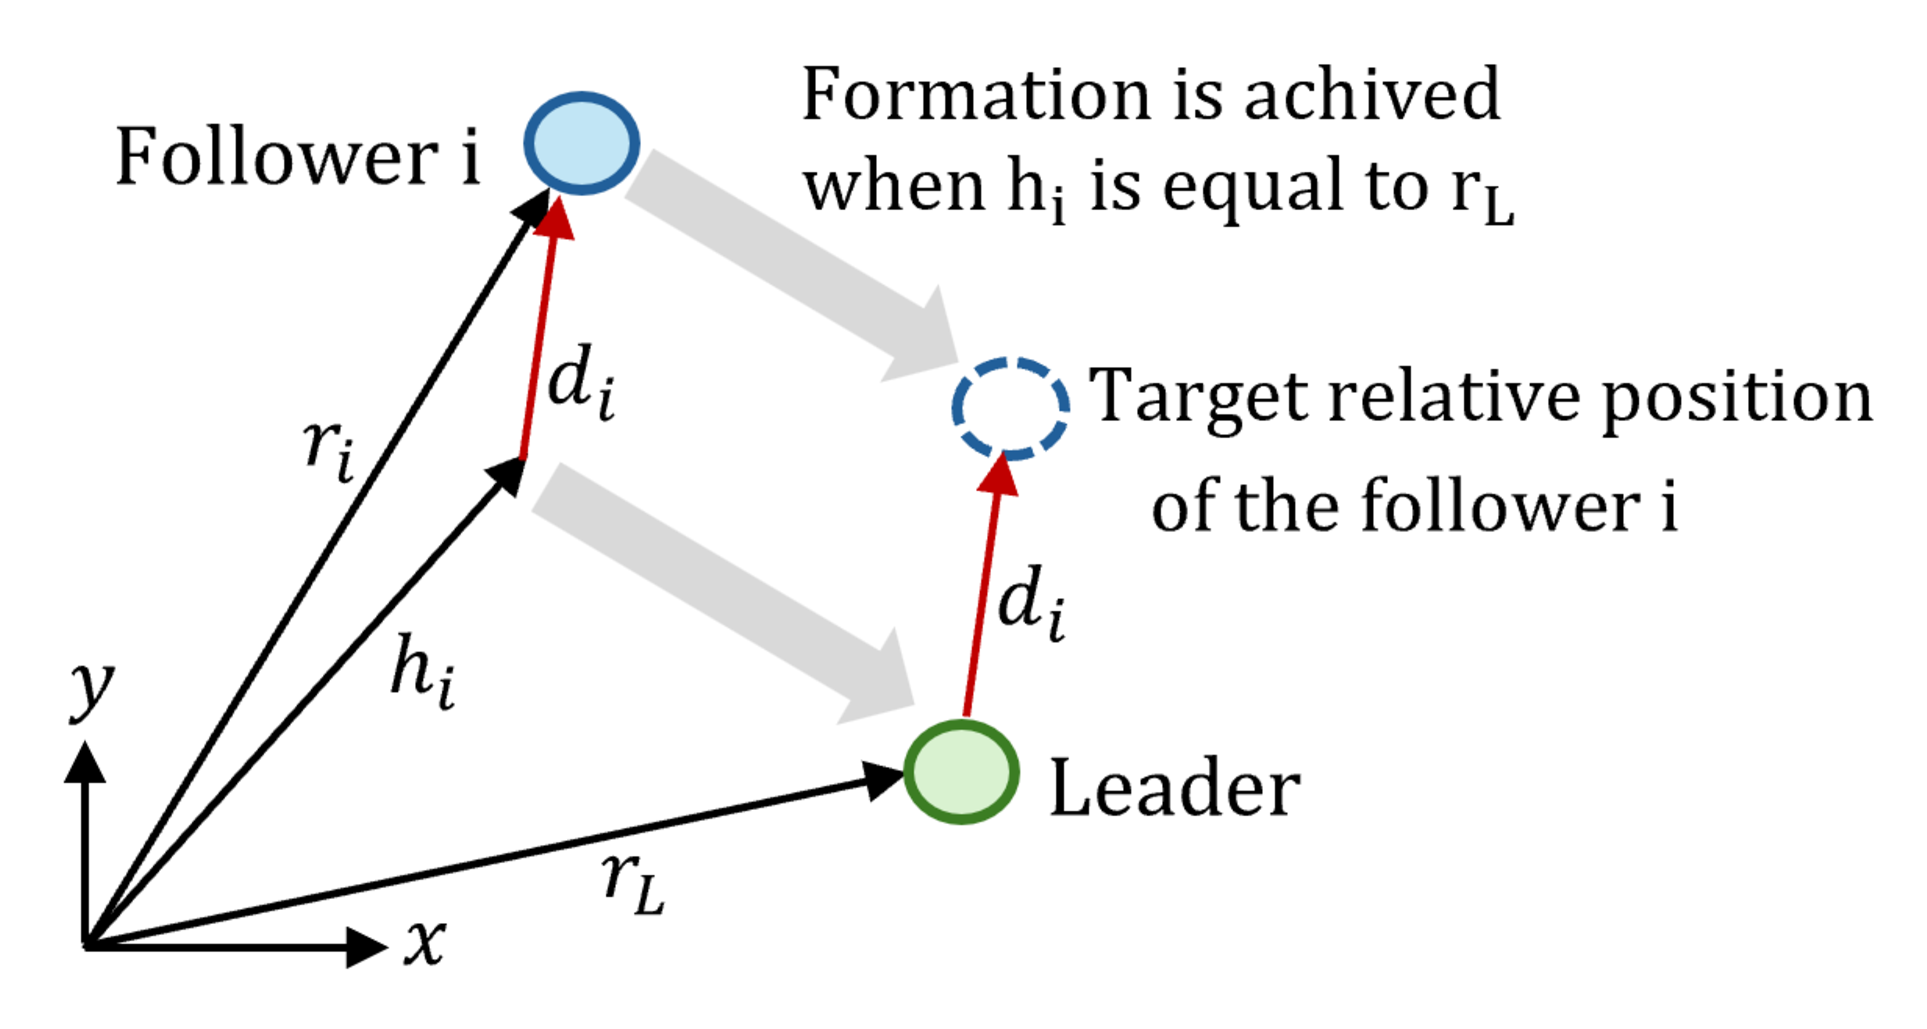
\includegraphics[width=\linewidth]{Fig/DefSymbol_(L-F).eps}
		\caption{Hierarchical likelihood.}
		\label{fig:hierarchical_likelihood}
	\end{center}
	\vspace{-2mm}
\end{figure}

First, for computational efficiency, the likelihood function is approximated by squared errors as:

\begin{equation}
\log p\left(T_{j}\right)=\sum_{k} e_{k}^{T} \Omega_{k} e_{k}
\end{equation}

Therefore, if some differentiable error $e^{k}$ can be obtained at each level, equation (38) can be computed. From equation (39), the derivative of the likelihood function can be calculated using the Gauss-Newton method as:

\begin{equation}
\begin{gathered}
\nabla_{T_{j}} \log p\left(T_{j}\right)=-\boldsymbol{\Psi}^{-1} \mathbf{b} \\
\boldsymbol{\Psi}=\mathbf{J}_{j}^{T} \mathbf{J}_{j}, \mathbf{b}=\mathbf{J}_{j}^{T} \mathbf{r}
\end{gathered}
\end{equation}

where the Jacobian $\mathbf{J}_{r}$ is calculated as:

\begin{equation}
\begin{aligned}
\mathbf{J}_{r} & =\left.\frac{\partial h\left(\varepsilon \boxplus T_{j}\right)}{\partial \varepsilon}\right|_{\varepsilon=0} \\
& =\left.\frac{\partial h}{\partial \varepsilon} \frac{\partial \varepsilon\left(\varepsilon \boxplus T_{j}\right)}{\partial \varepsilon}\right|_{\varepsilon=0} \\
& =\left.\sum_{k} \Omega_{k} e_{k}\left(T_{j}\right) \frac{\partial e_{k}\left(\varepsilon \boxplus T_{j}\right)}{\partial \varepsilon}\right|_{\varepsilon=0}
\end{aligned}
\end{equation}

\subsection{First Layer: Likelihood Using NetVLAD Features}
In the first layer, we use the similarity (distance) between the camera image observed at each step and past images registered in the database. Defining the similarity of NetVLAD features as $\omega_{j k}$ and the target pose obtained by the consensus algorithm as $T_{k}$, the error is defined as:

\begin{equation}
e_{k}=\left(T_{k}\right)^{-1} \otimes T_{j}, \quad \Omega_{k}=\omega_{j k}
\end{equation}

The derivative of the error from the differentiation on $\mathrm{SE}(3)$ is calculated as:

\begin{equation}
\begin{aligned}
\left.\frac{\partial e_{k}\left(\varepsilon \oplus T_{j}\right)}{\partial \varepsilon}\right|_{\varepsilon=0} & =\left.\frac{\partial\left(T_{k}\right)^{-1} e^{\varepsilon} T_{j}}{\partial \varepsilon}\right|_{\varepsilon=0} \\
& =\left[I_{4} \otimes R\left(\left(T_{k}\right)^{-1}\right)\right]\left.\frac{\partial e^{\varepsilon} T_{j}}{\partial \varepsilon}\right|_{\varepsilon=0} \\
& =\left(\begin{array}{cc}
\mathbf{0}_{3 \times 3} & -\mathbf{R}\left(T_{k}^{-1}\right) \mathbf{d}_{k}^{\wedge}\left(T_{j}\right) \\
\mathbf{R}\left(T_{k}^{-1}\right) & -\mathbf{R}\left(T_{k}^{-1}\right) \mathbf{d}_{k}^{\wedge}\left(T_{j}\right)
\end{array}\right)
\end{aligned}
\end{equation}

\subsection{Second Layer: Likelihood Using Feature Points}
In the second layer, corresponding points are matched, and the gradient is calculated by minimizing the distance between each pair. Defining the coordinates of Superpoint features in frame $i$ as $p_{i}$, the error is defined as:

\begin{equation}
e_{k}=T_{j} \oplus p_{j}-T_{k} \oplus p_{k}, \quad \Omega_{k}=\left(T_{j} \Sigma_{j}\left(T_{j}\right)^{\top}+T_{k} \Sigma_{k}\left(T_{k}\right)^{\top}\right)^{-1}
\end{equation}

The derivative of the error from the differentiation on $\mathrm{SE}(3)$ is calculated as:

\begin{equation}
\begin{aligned}
\left.\frac{\partial e_{k}\left(\varepsilon \oplus T_{j}\right)}{\partial \varepsilon}\right|_{\varepsilon=0} & =\left.\frac{\partial\left(e^{\varepsilon} T_{j}\right) \oplus p_{j}}{\partial \varepsilon}\right|_{\varepsilon=0} \\
& =\left(\mathbf{I}_{3}-\left[T_{j} \oplus p_{j}\right]^{\wedge}\right)
\end{aligned}
\end{equation}

\section{Simulations}
To verify the effectiveness of the proposed control methods, we conducted simulations using Algorithm 1. The simulation conditions are shown in Table \ref{tab:simulation_conditions}.

\begin{table}[b]
	\begin{center}
		\caption{Simulation conditions}
		\label{tab:simulation_conditions}
		\begin{tabular}{c c c} \hline
			Item & Parameter & Value \\ \hline
			Algorithm & Algorithm 1 & \\
			Number of agents & & 3 \\
			Particles per agent & & 50 \\
			Time steps & & 250 \\
			Total matches & & 250 \\
			Incorrect matches & & 52 \\
			Outlier ratio & & $\simeq 0.2$ \\ \hline
		\end{tabular}
	\end{center}
	\vspace{-1mm}
\end{table}

In the simulation, it is assumed that the relative position between random agent pairs (pseudo-closure loops, black dotted lines in Fig. \ref{fig:simulation}) is obtained at each step, and each agent's position is estimated using this relative information. It is also assumed that incorrect relative positions (red dotted lines in Fig. \ref{fig:simulation}) are obtained with a probability of about 0.2, and a collaborative self-localization simulation was conducted using matplotlib. The top left figure in Fig. \ref{fig:simulation} shows the true positions of each agent, and the top right, bottom left, and bottom right figures are the estimation screens for agents 1, 2, and 3, respectively. The incorrect relative positions were generated from random coordinates in the simulation area and the true positions of each agent.

\begin{figure}[t]
	\begin{center}
		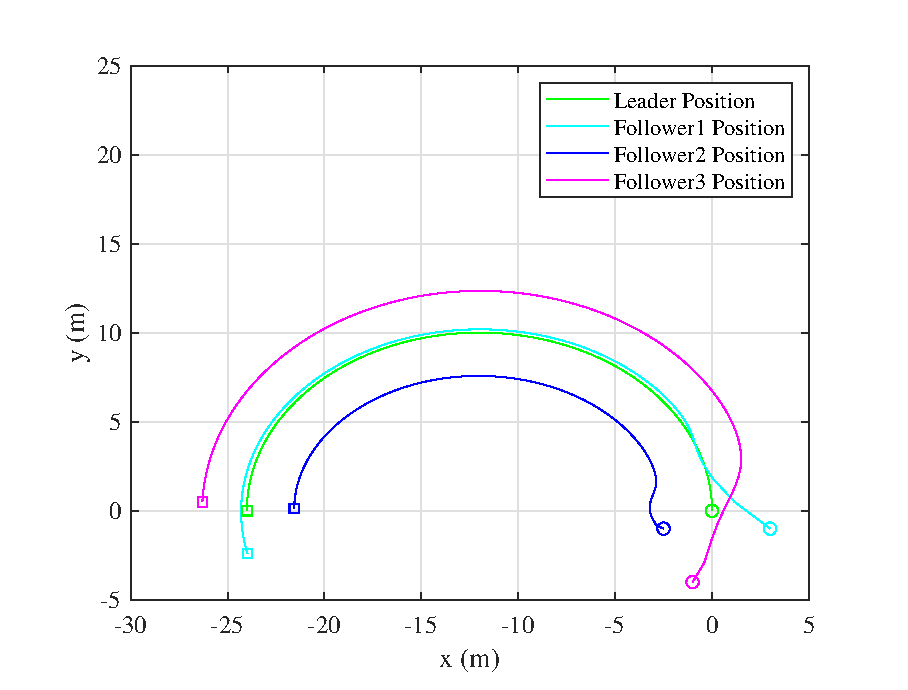
\includegraphics[width=\linewidth]{Fig/sampletrajectry.eps}
		\caption{Simulation (outlier ratio: 0.2, step: 0).}
		\label{fig:simulation}
	\end{center}
	\vspace{-2mm}
\end{figure}

\begin{figure}[t]
	\begin{center}
		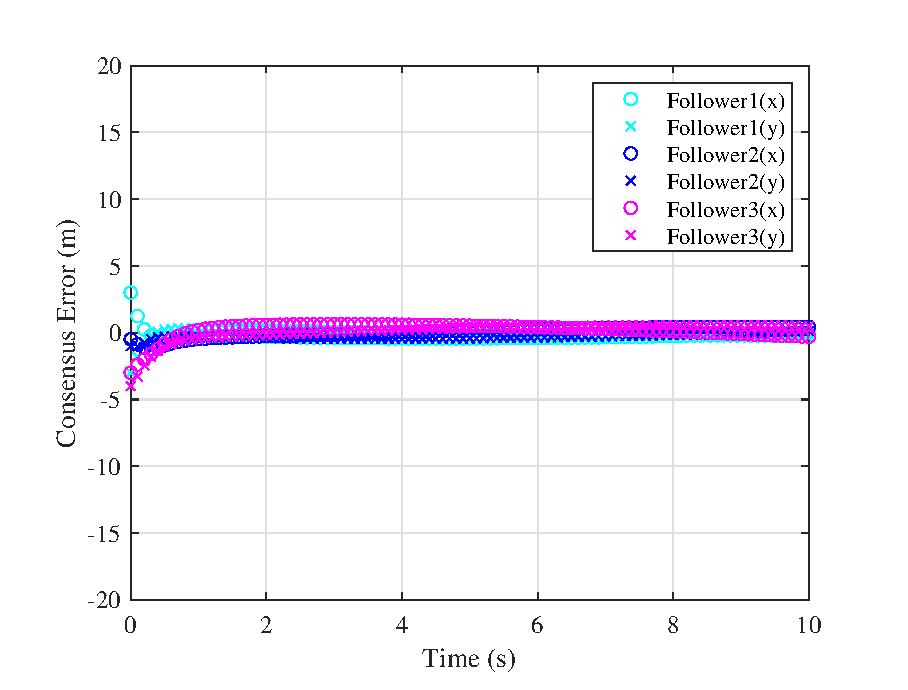
\includegraphics[width=\linewidth]{Fig/sampleconsensus.eps}
		\caption{Simulation (outlier ratio: 0.2, step: 150).}
		\label{fig:simulation_150}
	\end{center}
	\vspace{-2mm}
\end{figure}

Figs. \ref{fig:simulation} and \ref{fig:simulation_150} show the estimation states of each agent at 0 and 150 steps, respectively. From these, it can be seen that the probability distributions (particles), which were uniformly set at 0 steps, have converged to reasonable positions in all agent estimations at 150 steps. Also, Fig. \ref{fig:particle_transition} shows the time transition of the coordinates of all particles in the simulation. From Fig. \ref{fig:particle_transition} as well, it can be seen that consensus and convergence are achieved after about 150 steps.

\begin{figure}[t]
	\begin{center}
		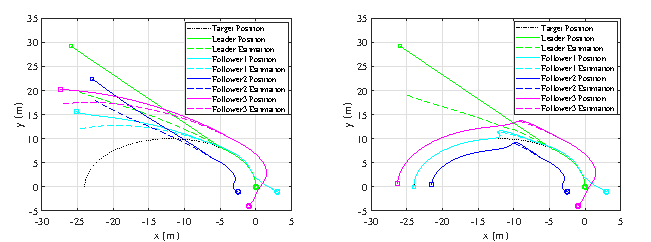
\includegraphics[width=\linewidth]{Fig/Leader_Trajectory_2ko1.eps}
		\caption{State transition of each particle (outlier ratio: 0.2).}
		\label{fig:particle_transition}
	\end{center}
	\vspace{-2mm}
\end{figure}

Next, as a stress test, we conducted simulations with increased probabilities of incorrect relative positions (outlier ratios). Figs. \ref{fig:particle_transition_05} and \ref{fig:particle_transition_08} show the time transitions of the coordinates of all particles in the cases where the outlier ratios are 0.5 and 0.8, respectively. From these, it can be seen that estimation is possible in the case of 0.5, but in the case of 0.8, the particles converge to incorrect coordinates.

\begin{figure}[t]
	\begin{center}
		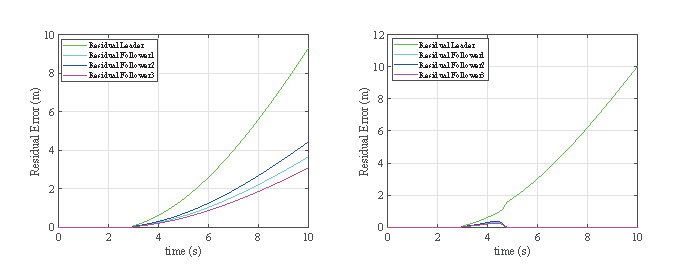
\includegraphics[width=\linewidth]{Fig/Leader_Residual_2ko1.eps}
		\caption{State transition of each particle (outlier ratio: 0.5).}
		\label{fig:particle_transition_05}
	\end{center}
	\vspace{-2mm}
\end{figure}

\begin{figure}[t]
	\begin{center}
		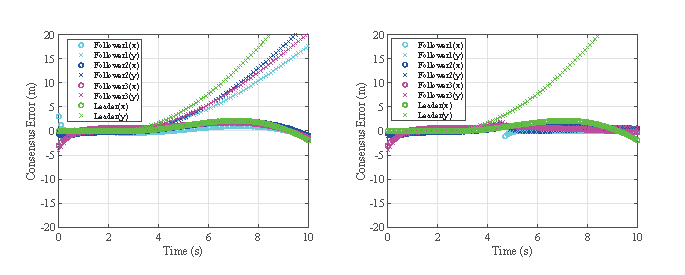
\includegraphics[width=\linewidth]{Fig/Leader_Consensus_2ko1.eps}
		\caption{State transition of each particle (outlier ratio: 0.8).}
		\label{fig:particle_transition_08}
	\end{center}
	\vspace{-2mm}
\end{figure}

\section{Real-World Experiments}
As a partial verification of the proposed method, we conducted real-world experiments with a single UAV equipped with a BMI270 IMU and an Intel RealSense D435 camera. In this experiment, it was observed that the Stein Particle Filter based on SVGD reduced error accumulation in 6 DoF state estimation and improved accuracy compared to benchmark methods (such as D2SLAM). While the full collaborative effect with multiple machines has not been verified, initial results have been obtained suggesting that the SPF-based framework proposed in this research may be useful in real-world environments. The conditions of the real-world experiments conducted are shown in Table \ref{tab:real_world_conditions}.

\begin{table}[b]
	\begin{center}
		\caption{Real-world experiment conditions}
		\label{tab:real_world_conditions}
		\begin{tabular}{c c c} \hline
			Item & Parameter & Value \\ \hline
			Number of agents & & 1 \\
			Number of particles & & 20 / agent \\
			Outlier ratio & & $\sim 10\%$ \\
			Ground Truth & & OptiTrack Flex3, Naturalpoint \\ \hline
		\end{tabular}
	\end{center}
	\vspace{-1mm}
\end{table}

Fig. \ref{fig:ros_experiment} shows the self-localization performed using ROS. Fig. \ref{fig:error_comparison} shows the error transition between each particle and the benchmark method with respect to the Ground Truth. From this, it can be confirmed that the proposed method can estimate with higher accuracy than the benchmark method for most of the time series. While the effectiveness of the gradient update method in 6 DoF has been verified by this experiment, future research aims to verify the consensus method with multiple machines.

\begin{figure}[t]
	\begin{center}
		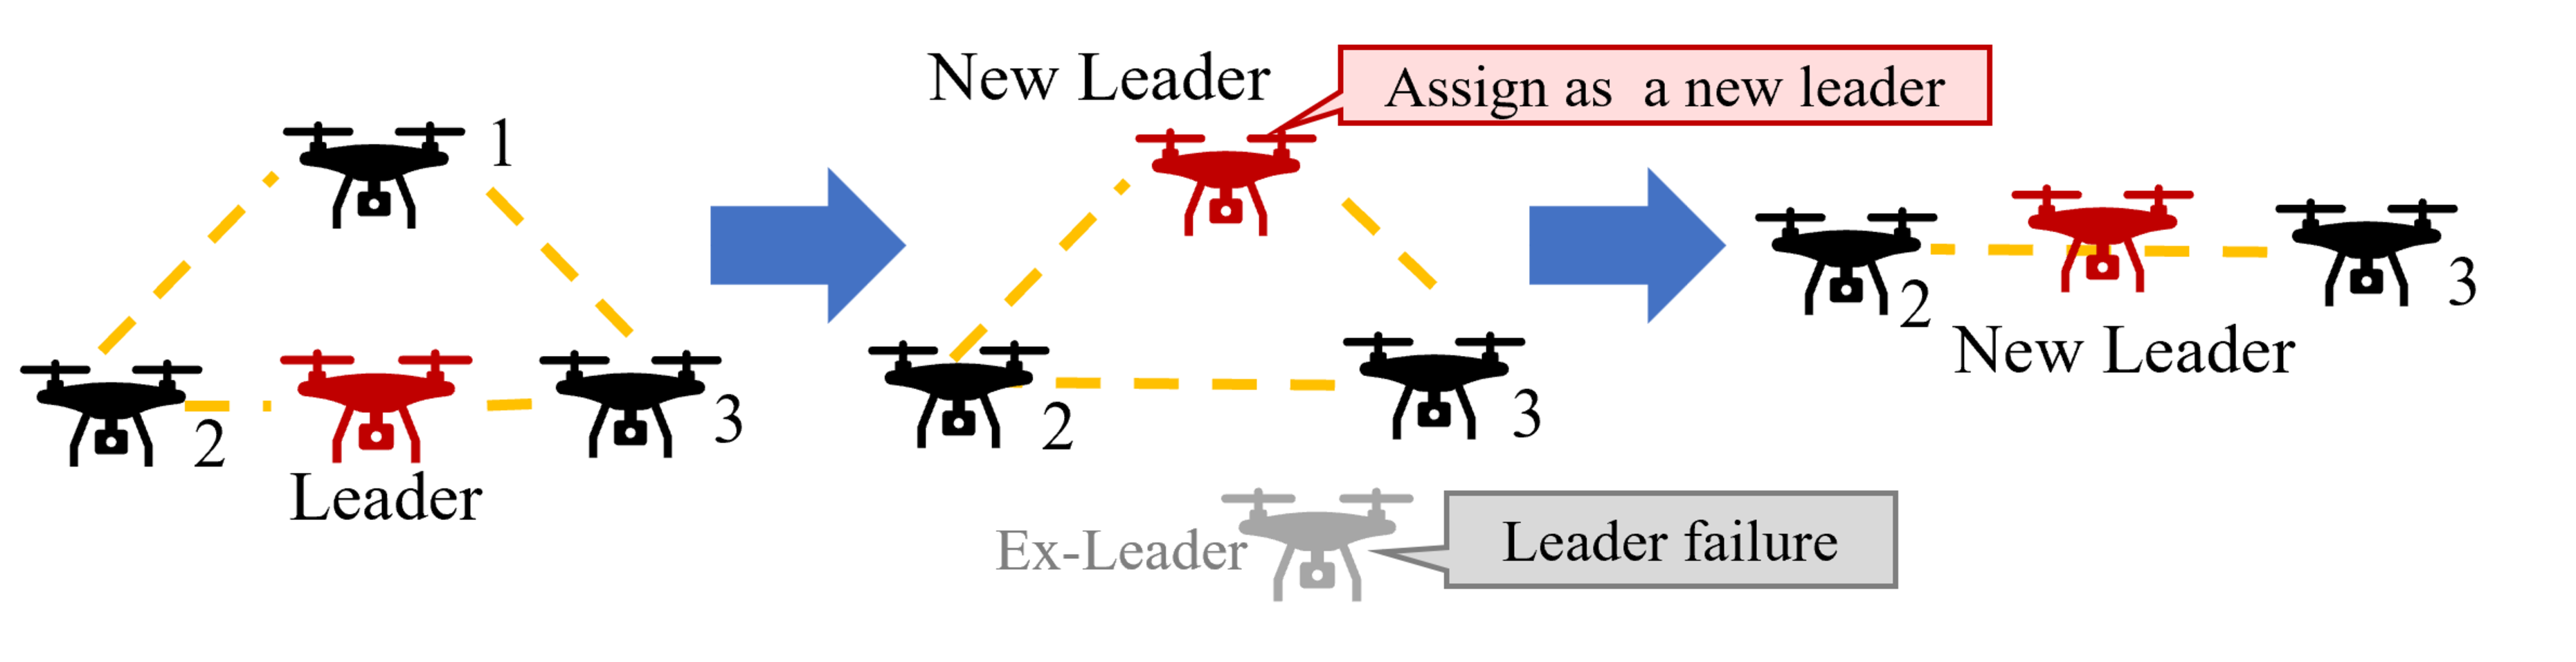
\includegraphics[width=\linewidth]{Fig/Nice_image_fault.eps}
		\caption{Verification of Stein Particle Filter using ROS.}
		\label{fig:ros_experiment}
	\end{center}
	\vspace{-2mm}
\end{figure}

\begin{figure}[t]
	\begin{center}
		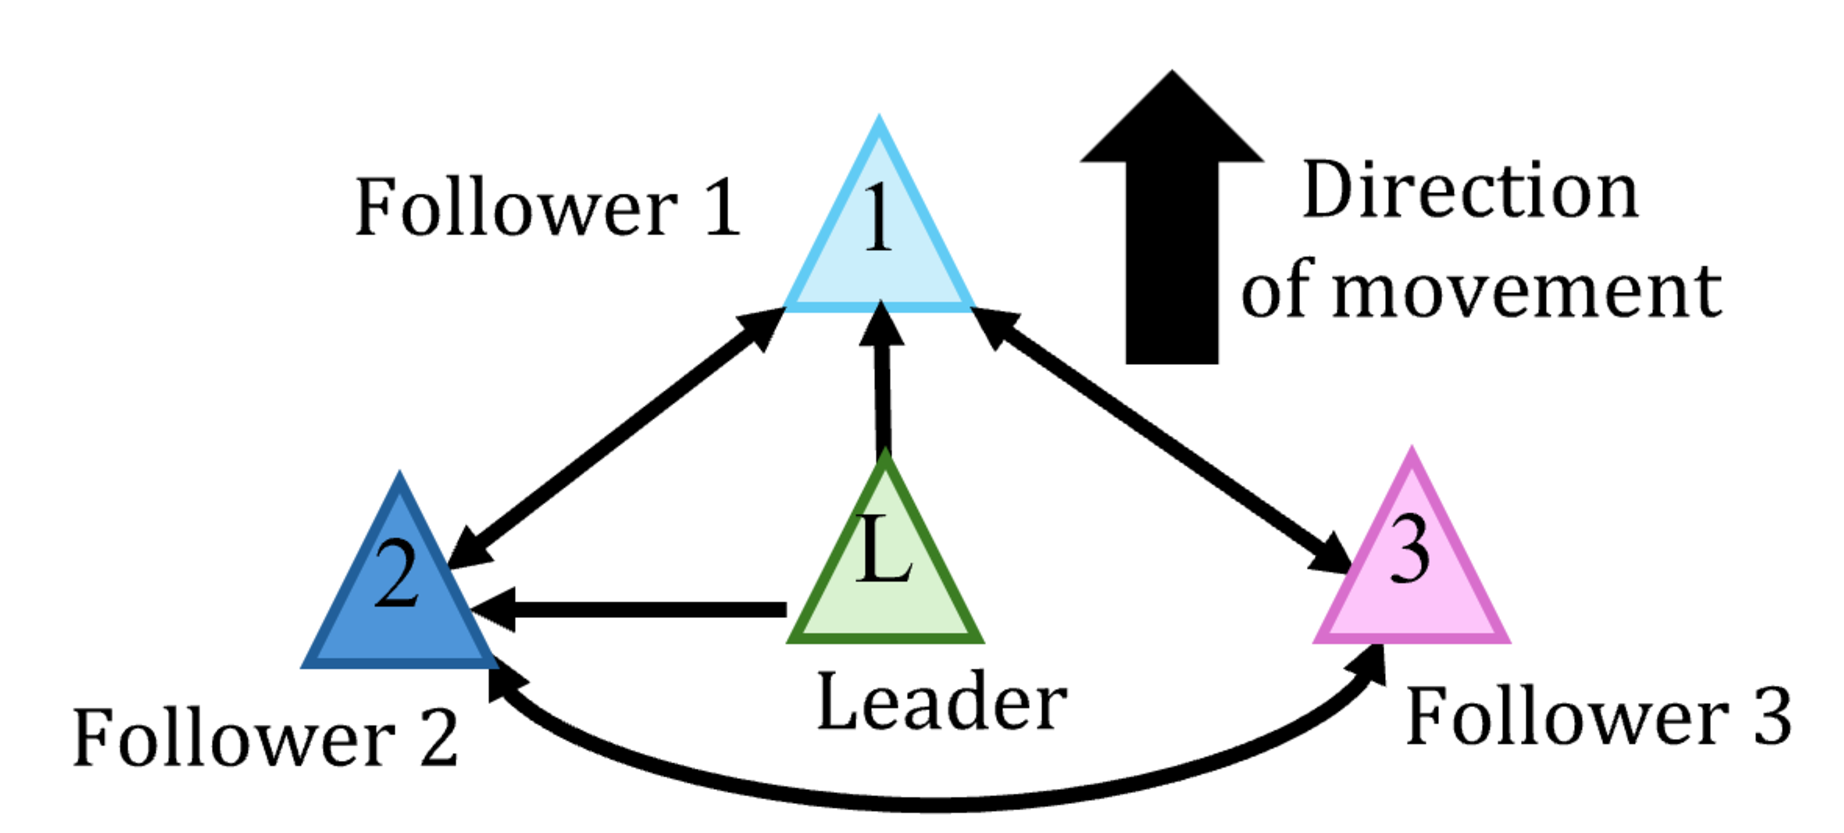
\includegraphics[width=\linewidth]{Fig/Topology.eps}
		\caption{Benchmark of Stein Particle Filter and D2SLAM.}
		\label{fig:error_comparison}
	\end{center}
	\vspace{-2mm}
\end{figure}

\section{Conclusions and Future Work}
In this paper, we proposed a new framework combining Stein Particle Filter and Relaxed ADMM, and addressed the problem of cooperative self-localization of UAVs in monotonous wide-area environments. The proposed method enables simultaneous handling of consensus constraints between multiple agents and multi-modal distributions, realizing stable position consensus in environments with outliers, which was difficult with conventional methods. Simulation and real-world experiment (single machine) results suggest that using SPF allows for more robust and flexible self-localization than existing methods by utilizing distribution approximation and gradient information. In the future, we plan to further verify the effectiveness and scalability of the proposed method through large-scale experiments with multiple UAVs at the real machine level.

\begin{thebibliography}{9}
\bibitem{VINS-Mono}T. Qin, P. Li, S. Shen, ``VINS-Mono: A Robust and Versatile Monocular Visual-Inertial State Estimator,'' {\it IEEE Transactions on Robotics}, Vol. 34, No. 4, pp. 1004-1020, 2018.

\bibitem{Multi-Robot-SLAM}W. Chen, X. Wang, S. Gao, G. Peng Shang, C. Zhou, Z. Li, C. Xu, K. Hu, ``Overview of Multi-Robot Collaborative SLAM from the Perspective of Data Fusion,'' {\it Machines}, 2023.

\bibitem{Swarm-Robots}X. Zhou, X. Wen, Z. Wang, Y. Gao, H. Li, Q. Wang, T. Yang, H. Lu, Y. Cao, C. Xu, F. Gao, ``Swarm of micro flying robots in the wild,'' {\it Science Robotics}, Vol. 7, No. 66, eabm5954, 2022.

\bibitem{Factor-Graphs}F. Dellaert, M. Kaess, ``Factor Graphs for Robot Perception,'' {\it Foundations and Trends in Robotics}, 2017.

\bibitem{VINS-IMU}M. Bloesch, M. Burri, S. Omari, M. Hutter, R. Siegwart, ``Iterated extended Kalman filter based visual-inertial odometry using direct photometric feedback,'' {\it The International Journal of Robotics Research}, Vol. 36, No. 9, pp. 1053-1072, 2017.

\bibitem{On-Manifold}C. Forster, L. Carlone, F. Dellaert, D. Scaramuzza, ``On-Manifold Preintegration for Real-Time Visual-Inertial Odometry,'' {\it IEEE Transactions on Robotics}, Vol. 33, No. 1, pp. 1-21, 2017.

\bibitem{SPF}F. A. Maken, F. Ramos, L. Ott, ``Stein Particle Filter for Nonlinear, Non-Gaussian State Estimation,'' {\it IEEE Robotics and Automation Letters}, Vol. 7, No. 2, pp. 5421-5428, 2022.

\bibitem{ADMM}N. Bastianello, M. Todescato, R. Carli, L. Schenato, ``Distributed Optimization over Lossy Networks via Relaxed Peaceman-Rachford Splitting: a Robust ADMM Approach,'' {\it Proc. of the 2018 European Control Conference (ECC)}, pp. 477-482, 2018.

\bibitem{SVGD}Q. Liu, D. Wang, ``Stein variational Gradient descent: a general purpose Bayesian inference algorithm,'' {\it Proc. of the 30th Int. Conf. on Neural Information Processing Systems}, pp. 2378-2386, 2016.

\bibitem{SE3-Tutorial}J.-L. Blanco, ``A tutorial on SE(3) transformation parameterizations and on-manifold optimization,'' 2012 [Online tutorial note].

\bibitem{MegaParticles}K. Koide, S. Oishi, M. Yokozuka, A. Banno, ``MegaParticles: Range-based 6-DoF Monte Carlo Localization with GPU-Accelerated Stein Particle Filter,'' {\it Proc. of IEEE International Conference on Robotics and Automation (ICRA)}, 2024.

\bibitem{NetVLAD}R. Arandjelovic, P. Gronat, A. Torii, T. Pajdla, J. Sivic, ``NetVLAD: CNN Architecture for Weakly Supervised Place Recognition,'' {\it IEEE Transactions on Pattern Analysis and Machine Intelligence}, Vol. 40, No. 6, pp. 1437-1451, 2018.

\bibitem{SuperPoint}D. DeTone, T. Malisiewicz, A. Rabinovich, ``SuperPoint: Self-Supervised Interest Point Detection and Description,'' {\it Proc. of the 2018 IEEE/CVF Conference on Computer Vision and Pattern Recognition Workshops (CVPRW)}, pp. 337-33712, 2018.

\bibitem{D2SLAM}H. Xu, P. Liu, X. Chen, S. Shen, ``$D^{2}$ SLAM: Decentralized and Distributed Collaborative Visual-Inertial SLAM System for Aerial Swarm,'' {\it IEEE Transactions on Robotics}, Vol. 40, pp. 3445-3464, 2024.
\end{thebibliography}

\end{document}
